\documentclass[twocolumn]{article}
%\documentclass{article}
\usepackage{fullpage}
% you really only need to use one of graphicx or epsfig
% there are example of using each one in this file
%\usepackage[dvips]{graphicx}
%usepackage{epsfig}
\usepackage{pgfplots}

% if you want two columns per page, but you also need to reformat the figures
% to span both columns if you do this
%\twocolumn
\begin{document}
\title{Testing Characteristics of the Linux Page Replacement Policy}

\author{Callen Rain \& Justin Cosentino}

\maketitle

\begin{abstract}
This paper describes some of the techniques used to identify the behavior of the Linux page replacement and discusses the implementation of a system call that provides page replacement statistics.  The system call provides page fault statistics for minor and major faults for a single process, processes grouped by owners, and all processes on the system. Several tests were developed that accessed large segments of memory on a Linux virtual machine. In each of the tests, access patterns exploited some page replacement scheme and favored others. An initial hypothesis of a Least Recently Used (LRU) algorithm was partially supported, although there was some evidence that the Linux implementation has characteristics resembling a working set. 
\end{abstract}

\section{Introduction}

We began 

 Describe at a high-level what you are doing and why, and describe what your high-level hypothesis is (i.e. "We started out guessing that Linux's page replacement policy is X, but our experiments will show that it is in fact, more like Y" or "we start out making no assumptions about Linux's page replacement policy, and our experiments will answer the question of is it more like X, Y or Z.").

\section{System Call}
Short paragraph describing how you implemented your system call to get get per-process, per-owner, and system wide page fault counts? Also, describe other Unix utilities you used to collect performance data for your experiments.

\section{Methodology}
\subsection{Experiments}
\subsubsection{Ruling Out Most Recently Used}
%--------------------------------------------%

\begin{figure}[h]
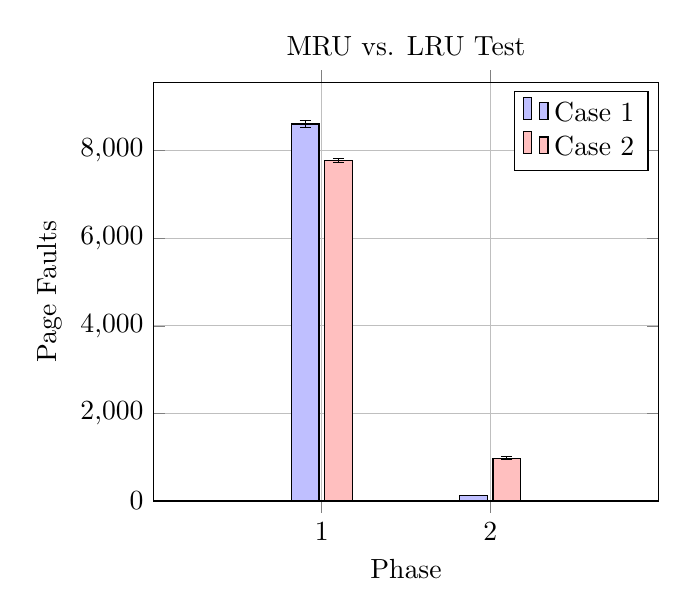
\begin{tikzpicture}
\begin{axis}[
    title = {MRU vs. LRU Test},
    width=8cm,
    xtick={1,...,2},
    xticklabels={1,2,3,4},
    grid=major,
    ybar, 
    bar width=10pt, 
    ylabel=Page Faults, 
    xlabel=Phase, 
    ymin=0, 
        enlarge x limits={abs=1}
    ]

\addplot[
    fill=blue!25,
    error bars/.cd,
        y dir=both,
        y explicit
] 
table [y error=error] {
x   y           error    label
1   8608.00 86.23 1
2   128.00 3.87 2
};

\addplot[
    fill=red!25,
    error bars/.cd,
        y dir=both,
        y explicit
] 
table [y error=error] {
x   y           error    label
1   7775.00   41.76 1
2   978.00   32.60 2
};
\legend{Case 1,Case 2}
\end{axis}
\end{tikzpicture}
\end{figure}

\begin{table}[h]
\begin{center}
\begin{tabular}{|c|c|r|r|}
\hline
{\bf Phase } & {\bf Case} & {\bf Page Faults} & {\bf Error } \\
\hline
1 & 1 & 8608.00 & $\pm$ 86.23 \\
& 2 & 7775.00 & $\pm$ 41.76 \\
\hline
2 & 1 & 128.00 & $\pm$ 3.87 \\
& 2 & 978.00 & $\pm$ 32.60 \\
\hline
\end{tabular}
\caption{ \label{rawio} MRU versus LRU test data
{\em  Description DescriptionDescriptionDescriptionDescription  }}
\end{center}
\end{table}

%--------------------------------------------%

\subsubsection{Ruling Out First In First Out}
%--------------------------------------------%
\begin{figure}[h]
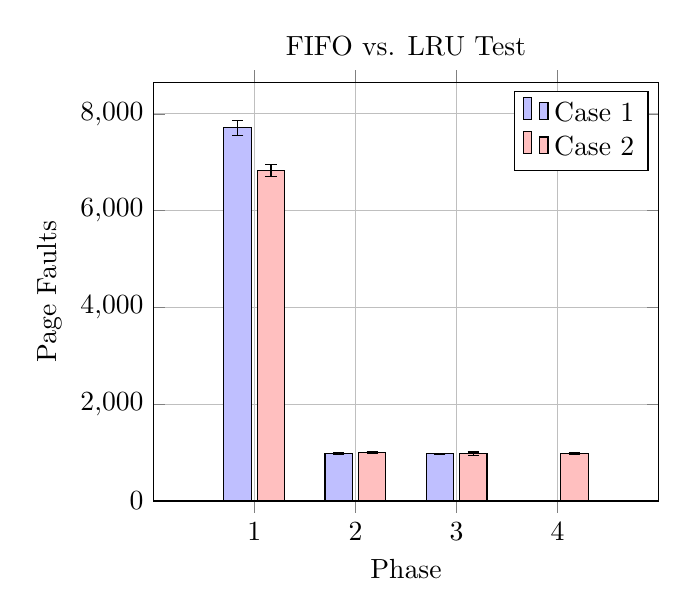
\begin{tikzpicture}
\begin{axis}[
    title = {FIFO vs. LRU Test},
    width=8cm,
    xtick={1,...,4},
    xticklabels={1,2,3,4},
    grid=major,
    ybar, 
    bar width=10pt, 
    ylabel=Page Faults, 
    xlabel=Phase, 
    ymin=0, 
    enlarge x limits={abs=1}
    ]

\addplot[
    fill=blue!25,
    error bars/.cd,
        y dir=both,
        y explicit
] 
table [y error=error] {
x   y           error    label
1   7708.00 158.27 1
2   976.00 20.27 2
3   976.00 8.89 3
4   0.00 0.00 4
};

\addplot[
    fill=red!25,
    error bars/.cd,
        y dir=both,
        y explicit
] 
table [y error=error] {
x   y           error    label
1   6832.00   128.12 1
2   993.00   20.12 2
3   979.00   33.21 3
4   983.00   15.59 4
};
\legend{Case 1,Case 2}
\end{axis}
\end{tikzpicture}
\end{figure}

\begin{table}[h]
\begin{center}
\begin{tabular}{|c|c|r|r|}
\hline
{\bf Phase } & {\bf Case} & {\bf Page Faults} & {\bf Error } \\
\hline
1 & 1 & 7708.00 & $\pm$ 158.27 \\
& 2 & 6832.00 & $\pm$ 128.12 \\
\hline
1& 1 & 976.00 & $\pm$ 20.27 \\
& 2 & 993.00 & $\pm$ 20.12 \\
\hline
2 & 1 & 976.00 & $\pm$ 8.89 \\
& 2 & 979.00 & $\pm$ 33.21 \\
\hline
1 & 1 & 0.00 & $\pm$ 0.00 \\
& 2 & 983.00 & $\pm$ 15.59 \\
\hline
\end{tabular}
\caption{ \label{rawio} FIFO versus LRU test data
{\em  Description  }}
\end{center}
\end{table}

%--------------------------------------------%

\subsubsection{Balance Between Working Set Least Recently Used}
%--------------------------------------------%
\begin{figure}[h]
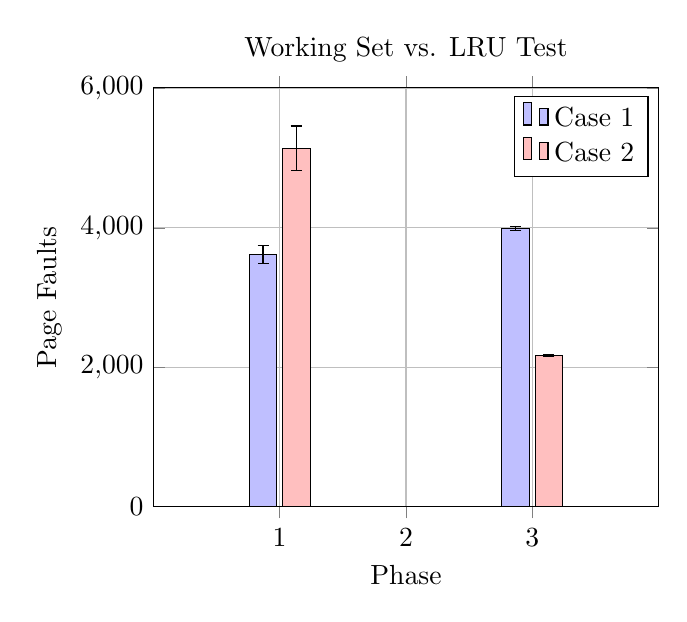
\begin{tikzpicture}
\begin{axis}[
    title = {Working Set vs. LRU Test},
    width=8cm,
    xtick={1,...,3},
    xticklabels={1,2,3,4},
    grid=major,
    ybar, 
    bar width=10pt, 
    ylabel=Page Faults, 
    xlabel=Phase, 
    ymin=0, 
    enlarge x limits={abs=1}
    ]

\addplot[
    fill=blue!25,
    error bars/.cd,
        y dir=both,
        y explicit
] 
table [y error=error] {
x   y           error    label
1   3614.00 131.24 1
2   1.00 1.00 2
3   3990.00 24.58 3
};

\addplot[
    fill=red!25,
    error bars/.cd,
        y dir=both,
        y explicit
] 
table [y error=error] {
x   y           error    label
1   5142.00   320.20 1
2   1.00   0.00 2
3   2163.00   13.96 3
};
\legend{Case 1,Case 2}
\end{axis}
\end{tikzpicture}
\end{figure}

\begin{table}[h]
\begin{center}
\begin{tabular}{|c|c|r|r|}
\hline
{\bf Phase } & {\bf Case} & {\bf Page Faults} & {\bf Error } \\
\hline
1 & 1 & 3614.00 & $\pm$ 131.24 \\
& 2 & 5142.00 & $\pm$ 320.20 \\
\hline
1& 1 & 1.00 & $\pm$ 1.00 \\
& 2 & 1.00 & $\pm$ 0.00 \\
\hline
2 & 1 & 3990.00 & $\pm$ 24.58 \\
& 2 & 2163.00 & $\pm$ 13.96 \\
\hline
\end{tabular}
\caption{ \label{rawio} Working Set versus LRU test data
{\em  Description  }}
\end{center}
\end{table}

%--------------------------------------------%

\subsubsection{Random LRU Behavior}

Main part: describe your experiments and results: For each experiment, you should:

Clearly state what your hypothesis is (i.e. "Application that does X should be a bad/good case for Linux's page replacement policy because ...)

Explain how your experiment is testing that hypothesis (We are testing this hypothesis by running application P, which does ..., N times on and collecting X,Y, and Z metrics using our system call, vmstat, time,... With these measures, we can see whether or not ... because ...).

Present your Results.

Explain your results! 
(Our results show that ... This does/does not match our expected result, because ... (if it doesn't, think about some other tests you could run to explain why it doesn't, or look for data you do have to explain it)

Quality of Experiments is much, much better than quantity; a few well thought out and well done experiments is sufficient.

\section{Conclusion}

It should include a statement of the major result(s) of your experiments (which policy(ies) is Linux's most like? and in what way(s)?). Also, tell me what you found to be the most difficult part of the hypothesis testing phase of this assignment.




\end{document}

